\documentclass[a4paper, 12pt]{article}
\usepackage[T2A,T1]{fontenc}
\usepackage[utf8]{inputenc}
\usepackage[english, russian]{babel}
\usepackage{graphicx}
\usepackage[hcentering, bindingoffset = 10mm, right = 13 mm, left = 13 mm, top=20mm, bottom = 20 mm]{geometry}
\usepackage{multirow}
\usepackage{lipsum}
\usepackage{amsmath, amstext}
\usepackage{siunitx}
\usepackage{subcaption}
\usepackage{wrapfig}
\usepackage{mathrsfs}
\usepackage{adjustbox}
\usepackage{enumerate, indentfirst, float}
\usepackage{capt-of, svg}
\usepackage{icomma}
\usepackage{xcolor}
\usepackage{ctable}
\usepackage{amssymb}
\usepackage[version=4]{mhchem}
\usepackage{expl3}
\usepackage{calc}


\newenvironment{bottompar}{\par\vspace*{\fill}}{\clearpage}
 
\begin{document}
\begin{titlepage}

\newcommand{\HRule}{\rule{\linewidth}{0.5mm}} % Defines a new command for the horizontal lines, change thickness here

\center % Center everything on the page
 
%----------------------------------------------------------------------------------------
%	HEADING SECTIONS
%----------------------------------------------------------------------------------------

\textsc{\LARGE Московский физико-технический институт\\(государственный университет)}\\[1,5cm] % Name of your university/college
\textsc{\Large Департамент молекулярной и биологической физики}\\[2cm] % Major heading such as course name
\textsc{\large Лабораторная работа}\\[0.5cm] % Minor heading such as course title

%----------------------------------------------------------------------------------------
%	TITLE SECTION
%----------------------------------------------------------------------------------------

\HRule
\\[0.2cm]
{ \huge \bfseries Электрокапиллярные явления.\\Свойства электродов}
\\[0.2cm] % Title of your document
\HRule
\\[1.5cm]


 
%----------------------------------------------------------------------------------------
%	AUTHOR SECTION
%----------------------------------------------------------------------------------------
\begin{minipage}{0.4\textwidth}
	\begin{flushleft}		
	\end{flushleft}
\end{minipage}
~
\begin{minipage}{0.4\textwidth}
	\begin{flushright} \large
		\emph{Авторы:}\\
		Светлана \textsc{Фролова} \\
		6113 группа \\
		Анатолий \textsc{Киселёв} \\
		6113 группа
	\end{flushright}
\end{minipage}


\begin{bottompar}
	\begin{center}
		
\includegraphics[width = 80 mm]{logo.jpg}
	\end{center}
	{\large г. Долгопрудный\\2018 г.}

\end{bottompar}
\vfill % Fill the rest of the page with whitespace

\end{titlepage}

\setcounter{page}{2}

\newpage
\section{Цели работы}
	\begin{enumerate}
	
		\item 
		Определение зависимости поверхностного натяжения на границе ртуть-раствор
электролита от электрического потенциала;
		\item 
		 Определение потенциала нулевого заряда и емкости двойного электрического
слоя на поверхности ртутного электрода в растворе;
		\item 
		 Исследование влияния природы электролита на потенциал нулевого заряда;
		\item 
		 Получение хлорсеребряного электрода;
		\item 
		 Исследование поляризуемости различных электродов. Выявление электродных процессов, ограниченных стадией массопереноса и стадией переноса заряда.
			
	\end{enumerate}
	
\section{Теоретическая часть}
Суть электрокапиллярных явлений заключается в изменении межфазного натяжения на поверхности раздела в результате ее заряжения. При постоянном составе электролита зависимость натяжения $\sigma$ от разности потенциалов $E$ определяется уравнением Липпмана:
\begin{equation}\label{lipman}
q=-\left(\frac{d\sigma}{dE}\right)_{\mu_i}
\end{equation}
Очевидно, что максимальное натяжение соответствует потенциалу, при котором
поверхность электрода не заряжена, так называемому потенциалу нулевого
заряда.\\

Если на поверхность ртути или другого металла нанести каплю органической
жидкости, нерастворимой в воде, то на трехфазной границе устанавливается
равновесие сил поверхностного натяжения в соответствии с уравнением Юнга:
\begin{equation}\label{sigma}
\sigma_{31}=\sigma_{32}+\sigma_{12}\cdot\cos{\theta}
\end{equation}
Это и позволяет исследовать изменение поверхностного натяжения на границе
раздела ртутный электрод-раствор электролита в зависимости от потенциала
электрода с помощью измерения краевого угла смачивания органической жидкости
$\theta$ (декана).

\subsection*{Поляризуемые и неполяризуемые границы раздела фаз}
Цели исследовании электродных процессов в электрохимии могут быть направлены на измерение как заряда, так и протекающего тока. Различия наглядно объясняются с помощью эквивалентнойй схемы Эршлера-Релндса

Она включает в себя три элемента: параллельно соединенные емкость двойного электрического слоя $C_\text{д.с.}$ и сопротивление фарадеевской реакции $\Theta$, последовательно к которым подключено омическое сопротивление в объеме раствора $R_\text{р}$. Величина фарадеевского сопротивления $\Theta$ обусловлена тем, что для протекания любого электрохимического процесса на электроде существует определенный энергетический барьер, подобный энергии активации для химических реакций. Для протекания заметного электрического тока и преодоления этого барьера необходимо прикладывать к электроду определенную величину так называемого перенапряжения. Если реакция идет трудно, величина сопротивления $\Theta$ велика и при незначительных приложенных напряжениях электрод ведет себя как конденсатор. Все приложенное напряжение идет на заряжение емкости двойного электрического слоя. В этом идеальном случае эквивалентная электрическая схема электрода представляет собой конденсатор $C_\text{д.с.}$ последовательно соединенный с резистором. Именно на таких, идеально поляризуемых, электродах принято изучать электрокапиллярные явления, описываемые уравнением Липпмана.

Другой крайний случай – электроды с очень низким сопротивлением реакции разряда $\Theta$. Они находятся в равновесии с продуктами электрохимической реакции и зарядить их поверхность с помощью внешних источников напряжения практически невозможно. В ответ на такую попытку возникает электрический ток, сбрасывающий «лишний» заряд. Такие, идеально неполяризуемые, электроды можно описать одним сопротивлением раствора $R_\text{р}$. Типичными представителями таких электродов, обладающих высокой плотностью тока обмена, являются все электроды сравнения. Их потенциал изменить с помощью внешнего напряжения практически невозможно.

\subsection*{}
\newpage
\section{Обработка результатов}
\subsection{Электроды}

По измеренным данным (таблица \ref{sigma31}) вычислим $\sigma_{31}$:\\

\begin{table}[h]
\centering
\caption{}
\label{sigma31}
\begin{tabular}{|c|c|c|c|c|}
\hline
$V, \text{мВ}$  & $d, \text{пиксели}$ & $h, \text{пиксели}$ & $\cos{\alpha}$     & $\sigma_{31},\text{мН/м}$\\ \hline
200   & 1261,051  & 366,488745 & 0,494943 & 400,2421  \\ \hline
100   & 1240,404  & 391,369391 & 0,430405 & 396,9506  \\ \hline
0     & 1257,955  & 361,864616 & 0,502635 & 400,6344  \\ \hline
-100  & 1285,172  & 363,309785 & 0,515539 & 401,2925  \\ \hline
-200  & 1377,192  & 307,470324 & 0,667531 & 409,0441  \\ \hline
-300  & 1479,684  & 267,226496 & 0,76919  & 414,2287  \\ \hline
-400  & 1523,607  & 255,237145 & 0,79815  & 415,7057  \\ \hline
-500  & 1521,316  & 255,158774 & 0,797715 & 415,6835  \\ \hline
-600  & 1452,697  & 255,237145 & 0,780183 & 414,7893  \\ \hline
-700  & 1483,683  & 277,218326 & 0,754934 & 413,5016  \\ \hline
-800  & 1431,294  & 287,294274 & 0,722416 & 411,8432  \\ \hline
-900  & 1379,192  & 311,04019  & 0,661898 & 408,7568  \\ \hline
-1000 & 1287,206  & 351,115366 & 0,541282 & 402,6054  \\ \hline
-1100 & 1261,032  & 365,034245 & 0,497928 & 400,3943  \\ \hline
-1200 & 1141,127  & 451,134126 & 0,230634 & 386,7624  \\ \hline
\end{tabular}
\end{table}

По формуле (\ref{sigma}) найдем $\sigma$ и построим график $\sigma(E)$.\\

\begin{figure}[!h]
	\centering
	\caption{}
	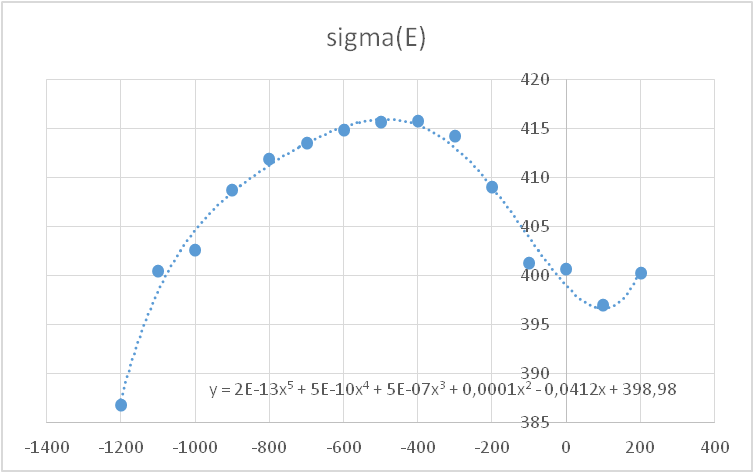
\includegraphics[width=0.8\textwidth]{image001.png}
\end{figure}
\newpage

По графику определим $\text{п.н.з} = -500\,\text{мВ}.$ \\
Из уравнения Липмана (\ref{lipman}) и второй производной $\frac{d^2\sigma}{dE^2}$ находим емкость двойного электрического слоя:
\[C_\text{д.с.}=0.3 \cdot 10^{-3} \textstyle\frac{\text{Ф}}{\text{м}^2}\]

Толщина двойного электрического слоя равна:
\[d=5,9 \cdot 10^{-8} \text{нм}\]

\subsection{Электрокапиллярность}
\subsubsection*{Получение и проверка работы хлорсеребряных электродов}

\begin{figure}[h!]
	\centering
	\caption{}	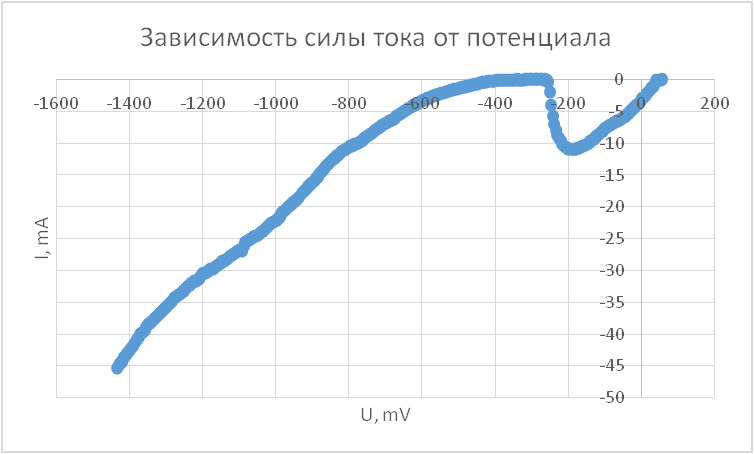
\includegraphics[width=0.7\textwidth]{image001(2).png}
\end{figure}

\begin{figure}[h!]
	\centering
	\caption{}	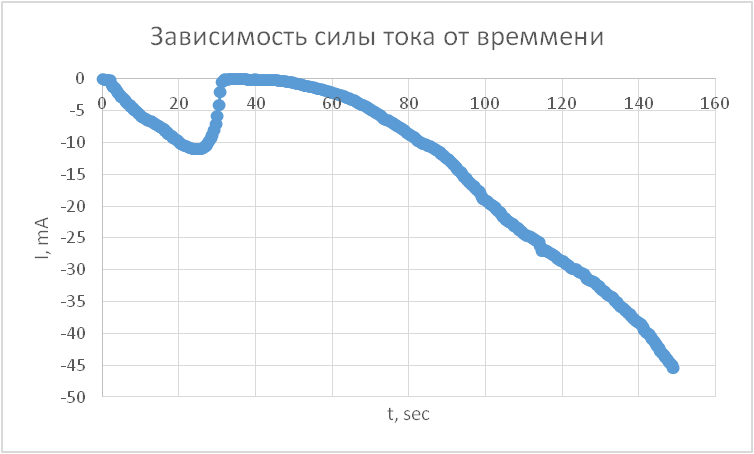
\includegraphics[width=0.7\textwidth]{image002.png}
\end{figure}

\newpage
\subsubsection*{Определение диффузионного потенциала}

\begin{minipage}{0.3\textwidth}
$$
\begin{array}{ccc}
	U_{\ce{HCl}} & = & 102 \\
	U_{\ce{KCl}} & = & 63 \\
	\Delta U & =  & 39 \\
\end{array}
$$
\end{minipage}
~
\begin{minipage}{0.3\textwidth}
$$
\begin{array}{ccc}
	\lambda_{\ce{K}} & = & 73,5 \\
	\lambda_{\ce{Cl}} & = & 76,35 \\
	\lambda_{\ce{H}} & =  & 349,8 \\
\end{array}
$$
\end{minipage}
~
\begin{minipage}{0.3\textwidth}

$$
\begin{array}{|c|c|}

	\hline	
	I &  U_{\text{диф}}\\
	\hline	
	0,1 & -0,00112\\
	\hline	
	1 & 0,037934\\
	\hline
\end{array}
$$
\end{minipage}


\subsubsection*{Циклическая вольт-амперометрия}


\begin{figure}[h!]
	\centering
	\caption{}	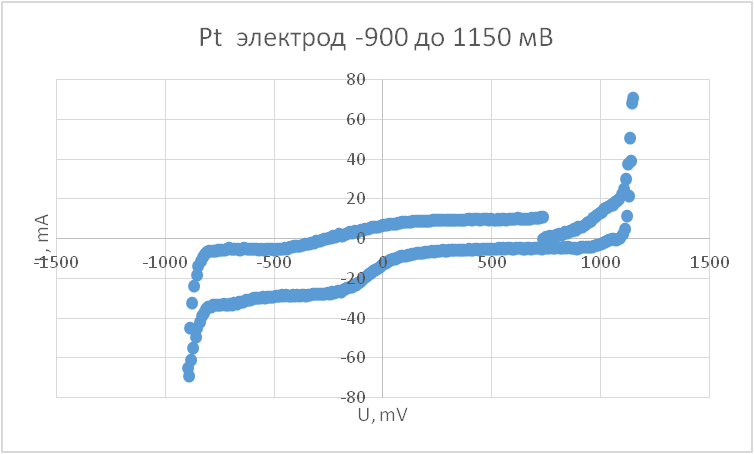
\includegraphics[width=0.8\textwidth]{image004.png}
\end{figure}

\begin{figure}[h!]
	\centering
	\caption{}	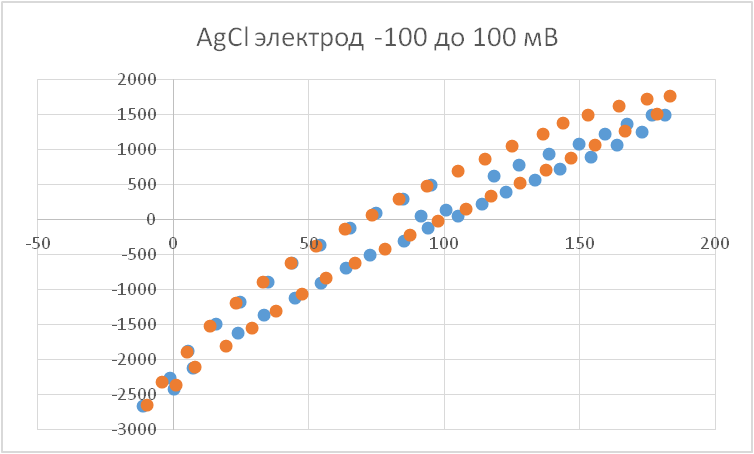
\includegraphics[width=0.8\textwidth]{image006.png}
\end{figure}


\begin{figure}[h!]
	\centering
	\caption{}	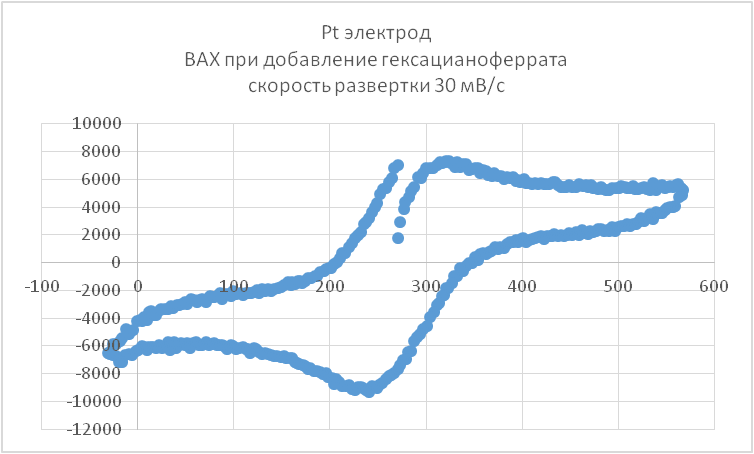
\includegraphics[width=0.8\textwidth]{image008.png}
\end{figure}

\newpage

\begin{figure}[h!]
	\centering
	\caption{}	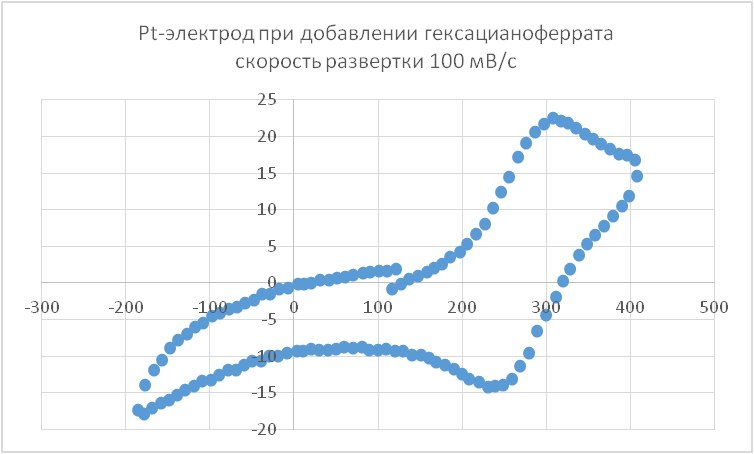
\includegraphics[width=0.8\textwidth]{image010.png}
\end{figure}


\begin{figure}[h!]
	\centering
	\caption{}	
\includegraphics[width=0.8\textwidth]{image012.png}
\end{figure}

\newpage

\subsubsection*{Поляризуемые и неполяризуемые электроды, стационарные кривые поляризации для Ox-Red электрода}


\begin{figure}[h!]
	\centering
	\caption{}	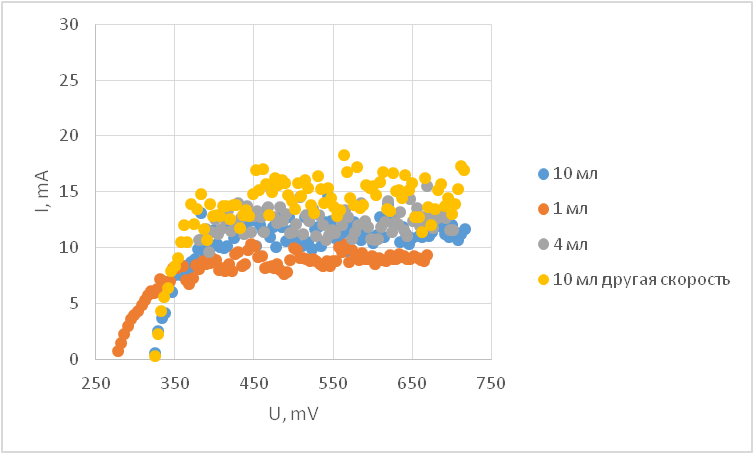
\includegraphics[width=0.8\textwidth]{image014.png}
\end{figure}

\newpage

\subsubsection*{Коррозия}


\begin{figure}[h!]
	\centering
	\caption{}	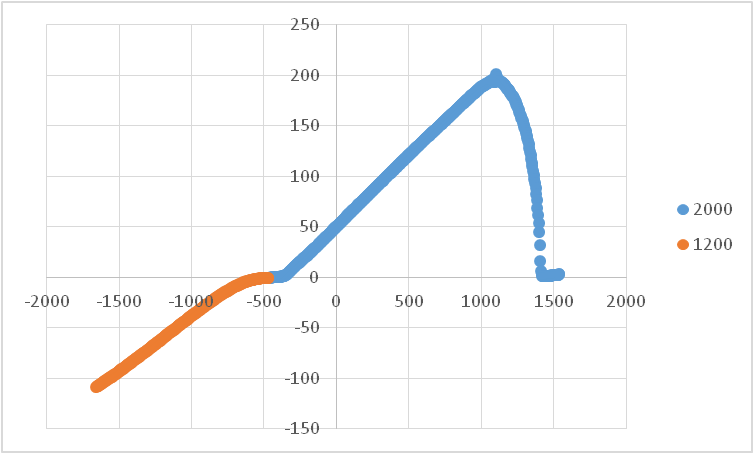
\includegraphics[width=0.8\textwidth]{image017.png}
\end{figure}

\newpage
\section{Вывод}
Мы определили зависимость поверхностного натяжения на границе ртуть-раствор электролита от электрического потенциала, нашли потенциал нулевого заряда и емкость двойного электрического слоя на поверхности ртутного электрода в растворе. Также исследовали влияние природы электролита на потенциал нулевого заряда, получили хлорсеребряный электрод и исследовали поляризуемости различных электродов.

\end{document}